\documentclass{article}
\usepackage[T1]{fontenc}
\usepackage{amssymb, amsmath, graphicx, subfigure, enumerate}
\usepackage{amsthm,alltt} 
\usepackage[margin=1.25in]{geometry} %geometry (sets margin) and other useful packages
\usepackage{graphicx,ctable,booktabs}
\usepackage{mathtools}
\usepackage[boxed]{algorithm2e}
\usepackage{mathdots}
\usepackage{fancyhdr} %Fancy-header package to modify header/page numbering
\usepackage{cleveref}

\setlength{\oddsidemargin}{.25in}
\setlength{\evensidemargin}{.25in}
\setlength{\textwidth}{6in}
\setlength{\topmargin}{-0.4in}
\setlength{\textheight}{8.5in}

\newcommand{\heading}[6]{
  \renewcommand{\thepage}{\arabic{page}} % used to be #1-\arabic{page}
  \noindent
  \begin{center}
  \framebox{
    \vbox{
      \hbox to 5.78in { \textbf{#2} \hfill #3 }
      \vspace{4mm}
      \hbox to 5.78in { {\Large \hfill #6  \hfill} }
      \vspace{2mm}
      \hbox to 5.78in { \textit{Instructor: #4 \hfill #5} }
    }
  }
  \end{center}
  \vspace*{4mm}
}

%Redefining sections as problems
\makeatletter
\newenvironment{problem}{\@startsection
       {section}
       {2}
       {-.2em}
       {-3.5ex plus -1ex minus -.2ex}
       {2.3ex plus .2ex}
       {\pagebreak[3]%forces pagebreak when space is small; use \eject for better results
       \large\bf\noindent{Problem }
       }
       }
       %{%\vspace{1ex}\begin{center} \rule{0.3\linewidth}{.3pt}\end{center}}
       %\begin{center}\large\bf \ldots\ldots\ldots\end{center}}
\makeatother


\newtheorem{theorem}{Theorem}[section]
\newtheorem{definition}[theorem]{Definition}
\newtheorem{remark}[theorem]{Remark}
\newtheorem{lemma}[theorem]{Lemma}
\newtheorem{corollary}[theorem]{Corollary}
\newtheorem{proposition}[theorem]{Proposition}
\newtheorem{claim}[theorem]{Claim}
\newtheorem{observation}[theorem]{Observation}
\newtheorem{fact}[theorem]{Fact}
\newtheorem{assumption}[theorem]{Assumption}

% don't modify this unless you know what you're doing
\newcommand{\problemset}[3]{\heading{#1}{\classname: Machine Learning for Trading}{#2}{Tucker Balch}{#3}{Assignment 1 - Report}}


%%%%%%%% ENTER YOUR INFORMATION HERE %%%%%%%%
\newcommand{\problemsetnum}{1}            % problem set number
\newcommand{\duedate}{August 30, 2018} % problem set deadline
\newcommand{\studentname}{Seyma Gurkan}      % name of student (i.e., you)
\newcommand{\classname}{CS 7646}
%%%%%%%%%%%%%%%%%%%%%%%%%%%%%%%%%%%%%%%%%%%%%

\pagestyle{fancy}
%\addtolength{\headwidth}{\marginparsep} %these change header-rule width
%\addtolength{\headwidth}{\marginparwidth}
\lhead{\classname} %Problem \thesection}
\chead{} 
\rhead{\thepage} 
\lfoot{\small\scshape \classname}
\cfoot{} 
\rfoot{\footnotesize PS \#\problemsetnum} 
\renewcommand{\headrulewidth}{.3pt} 
\renewcommand{\footrulewidth}{.3pt}
\setlength\voffset{-0.25in}
\setlength\textheight{648pt}


\newcommand{\sit}{\shortintertext}
\newcommand\deq{\mathrel{\overset{\makebox[0pt]{\mbox{\normalfont\tiny\sffamily def}}}{=}}}
\newcommand{\ones}{\mathbbm{1}}
\newcommand{\e}{\vec{e}}
\newcommand{\tr}{\text{tr}}
\newcommand{\bs}{\boldsymbol}
\mathchardef\mhyphen="2D
\newcommand{\C}{\mathbb{C}}
\newcommand{\R}{\mathbb{R}}

\newcommand{\vol}{\text{vol}}

\renewcommand{\thesubsection}{\thesection.\alph{subsection}}


% auto sized delimiters

\newcommand{\br}[1]{\left[#1\right]}
\newcommand{\pr}[1]{\left(#1\right)}
\newcommand{\ceil}[1]{\left\lceil#1\right\rceil}
\newcommand{\floor}[1]{\left\lfloor#1\right\rfloor}
\newcommand{\abs}[1]{\left|#1\right|}
%default delimiter for Pr and E
\DeclarePairedDelimiter{\defaultDelim}{[}{]}

\DeclareMathOperator{\capPr}{Pr}
\renewcommand{\Pr}[2][]{\capPr_{#1}\defaultDelim*{#2}}
\DeclareMathOperator{\capE}{E}
\newcommand{\E}[2][]{\capE_{#1}\defaultDelim*{#2}}
\DeclareMathOperator{\capVar}{Var}
\newcommand{\Var}[2][]{\capVar_{#1}\defaultDelim*{#2}}

%\DeclareMathOperator*{}{} puts subscript below
 \renewcommand{\baselinestretch}{1.3}

%%%%%%%%%%%%%%%%%%%%%%%%%%%%%%%%%%%%%%%%%%%%%%%%%
\begin{document}
\problemset{\problemsetnum}{\duedate}{\studentname}

\underline{\textbf{Question 1}}
\\
\\
We can claim that it is almost surely equal to 1, since we don't have lower bound for betting. As it also be seen from Figure 1, standard deviation for the winnings is approaches to zero while number of bets increases. Approximately after 200 iterations, we see that winning is equal to \$80 almost surely.
\\

\underline{\textbf{Question 2}}
\\
\\
From Figure 2, we can see that mean of the winning is equal to 80 after 200 bets with almost zero standard deviation. Therefore, expected value of our winnings is equal to 80. 
\\

\underline{\textbf{Question 3}}
\\
\\
Yes the standard deviation reaches to a maximum value then converges as the number of sequential bets increases. The reason that standard deviation that high is that bet amount do not have a bound, and it we can have a huge gain or lost due to this factor. However, once we reach to \$80 as episode winning, then we don't bet anymore, and winning is constant as this value. Due to the structure of betting, we definitely reach to this level after first certain number of iterations. Then, standard deviation converges to zero.
\\

\underline{\textbf{Question 4}}
\\
It is equal to $18/38$, which is the winning probability for each individual game.
\\

\underline{\textbf{Question 5}}
\\
\\
From Figure 4, we can conclude that it is very close to -50. At the end 1000 episodes, we have only two probabilities for the winnings. It is either 80 or -256. 
\\

\underline{\textbf{Question 6}}
\\
\\
To answer this question, we can get some help from Figure 4. This time standard deviation increases with the sequential betting. Even though it stabilizes as the bet number increases, it does not converge to 0 this time.This time in converges slower compared to experiment 1. From the Figure, we can tell that std. dev. converges around 150. The reason for this, there are two options for winnings to converge. It is either 80 or -256. Therefore, each simulation ends up with one of that. This causes to a positive standard deviation. 
\\

\underline{\textbf{Question 7}}
\\
\\
The figures can be seen from Figure 1 through Figure 5. 
\begin{figure}
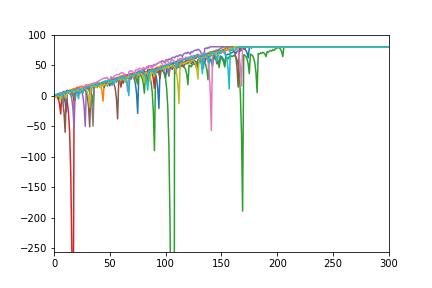
\includegraphics[]{plot.png}
\caption{The result when simulator is run 10 times}
\end{figure}
\begin{figure}
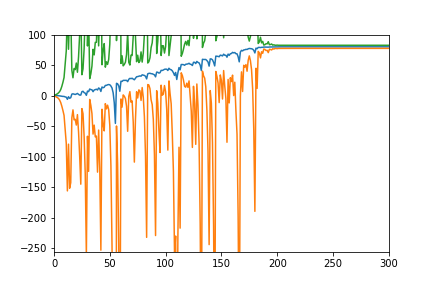
\includegraphics[]{plot2.png}
\caption{The mean plot when simulator is run 1000 times}
\end{figure}
\begin{figure}
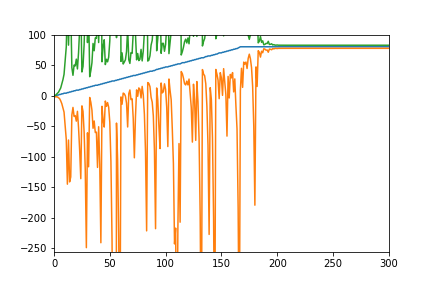
\includegraphics[]{plot3.png}
\caption{The median plot when simulator is run 1000 times}
\end{figure}
\begin{figure}
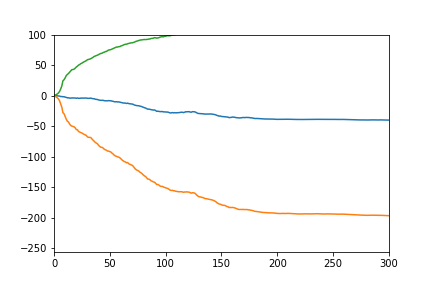
\includegraphics[]{plot4.png}
\caption{The mean plot for the experiment 2}
\end{figure}
\begin{figure}
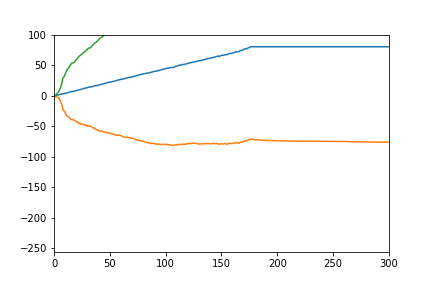
\includegraphics[]{plot5.png}
\caption{The median plot for the experiment 2}
\end{figure}




















\end{document}